\section{de Giorgi lemma}\label{DeGiorgiSection}
In this section we prove a generalization, Proposition \ref{de Giorgi lemma}, of the de Giorgi lemma.
The euclidean version of this lemma \cite[Teorema 5.7]{Miranda66} is to prove that the reduced boundary of a set of least perimeter in smooth \cite[Teorema 6.4]{Miranda66}.

\subsection{Multilinear computations}
Before we state the de Giorgi lemma we carry out some computations in multilinear algebra which we will use to estimate the surface area of $\partial^* U$.
We remind the reader of our conventions for Einstein summation, Notation \ref{EinsteinNotation}.

Suppose that we are given a $d$-dimensional oriented real Hilbert space $(\Hilb, g)$, and an oriented basis $(\partial_0, \dots, \partial_{d - 1})$ which may not be orthonormal but which satisfies for every $i$
\begin{equation}\label{0th coordinate orthogonal}
g_{0i} = 0
\end{equation}
where $g_{\mu\nu} = g(\partial_\mu, \partial_\nu)$.
We write $g_{\hat 0 \hat 0}$ for the inner product on the span $\Hilb_0^\perp$ of $\partial_1, \dots, \partial_{d - 1}$ defined by $(g_{\hat 0 \hat 0})_{ij} = g_{ij}$.
We as usual write $g^{\mu\nu}$, $(g^{\hat 0 \hat 0})^{ij}$ for the components of the dual metric, and $\delta_\mu^\nu$ for the components of the identity matrix.

\begin{definition}
The \dfn{Gramian matrix} of $v_1, \dots, v_{d - 1}$ is
$$\Gram(v_1, \dots, v_{d - 1})_{ij} = g_{\mu \nu} v_i^\mu v_j^\nu.$$
The \dfn{cross product} $v_1 \times \cdots \times v_{d - 1}$ of vectors $v_1, \dots, v_{d - 1} \in \Hilb$ is defined to be the vector $v_0$
such that:
\begin{enumerate}
\item $g(v_0, v_i) = 0$,
\item $((-1)^{d - 1} v_0, v_1, \dots, v_{d - 1})$ is positively oriented, and
\item the length is
$$|v_0|_g^2 = |\det \Gram(v_1, \dots, v_{d - 1})|.$$
\end{enumerate}
\end{definition}

Here the orientation convention is chosen so that if $\partial_0, \dots, \partial_{d - 1}$ is an orthonormal basis, thus $g_{\mu\nu} = \delta_{\mu\nu}$, then the cross product is computed by the formal determinant
\begin{equation}\label{formal determinant}
v_1 \times \cdots \times v_{d - 1} = \begin{vmatrix}\partial_0 & \cdots & \partial_{d - 1} \\
v_1^0 & \cdots & v_1^{d - 1}\\
& \vdots \\
v_{d - 1}^0 & \cdots & v_{d - 1}^{d - 1}\end{vmatrix}
\end{equation}
which of course agrees with the orientation convention of the cross product on $\RR^3$.

\begin{lemma} \label{cross product formula}
Suppose that $\phi_1, \dots, \phi_{d - 1} \in \Hilb$ satisfy $\phi_i^0 = \psi_i$, $\phi_i^j = \delta_i^j$ for some $\psi \in (\Hilb_0^\perp)'$.
Let $h_{ij} = (g_{00})^{-1} g_{ij}$, and let $\normal \in \Hilb'$ be the unit covector which annihilates $\phi_1, \dots, \phi_{d - 1}$ with $((-1)^{d - 1}\normal^\sharp, \phi_1, \dots, \phi_{d - 1})$ positively oriented.
Then
\begin{align}
|\det \Gram(\phi_1, \dots, \phi_{d - 1})| &= (g_{00})^{d - 1} (1 + |\psi|_{h^{-1}}^2) \det h, \label{WeinsteinAronszajn} \\
(\phi_1 \times \cdots \times \phi_{d - 1})^\mu &= (g_{00})^{d/2} g^{\mu \nu}(\delta_\nu^0 - \delta^i_\nu \psi_i) \sqrt{\det h}, \label{CrossProduct} \\
\normal_\mu &= \sqrt{\frac{g_{00}}{1 + |\psi|_{h^{-1}}^2}} (\delta^0_\mu - \delta^i_\mu \psi_i) \label{conormal crossproduct}.
\end{align}
\end{lemma}
\begin{proof}
We begin by computing
$$\Gram(\phi_1, \dots, \phi_{d - 1})_{ij} = g_{\mu \nu} \phi_i^\mu \phi_j^\nu = g_{00} \psi_i \psi_j + g_{ij}$$
which are the components of $g_{00}\psi \otimes \psi + g_{\hat 0 \hat 0} \in (\Hilb_0^\perp \otimes \Hilb_0^\perp)'$.
By the Weinstein-Aronszajn theorem \cite{Tao13}, $\det(1 + h^{-1}(\psi \otimes \psi)) = 1 + |\psi|_{h^{-1}}^2$, so
\begin{align*}
\det(g_{00}\psi \otimes \psi + g_{\hat 0 \hat 0})
&= (g_{00})^{d - 1} \det(\psi \otimes \psi + h) = (g_{00})^{d - 1} \det(h^{-1}(\psi \otimes \psi) + 1) \det h \\
&= (g_{00})^{d - 1} (1 + |\psi|_{h^{-1}}^2) \det h.
\end{align*}
Since $h$ is a quadratic form of signature $(+, \cdots, +)$, its determinant is positive and so (\ref{WeinsteinAronszajn}) holds.

We begin the proof of (\ref{CrossProduct}) by checking orthogonality:
\begin{align*}
g_{\mu\nu} g^{\mu \lambda} (\delta^0_\lambda - \delta^i_\lambda \psi_i)(\delta^\nu_0 \psi_i + \delta^\nu_i)
&= \delta^\lambda_\nu (\delta^0_\lambda - \delta^i_\lambda \psi_i)(\delta^\nu_0 \psi_i + \delta_i^\nu)
= \psi_i - \psi_i = 0.
\end{align*}
To check orientation we may assume that $g_{\mu\nu} = \delta_{\mu\nu}$ in which case we just need to check agreement with (\ref{formal determinant}):
$$\begin{vmatrix} \partial_0 && \cdots && \partial_{d - 1} \\
\psi_1 & 1 & 0 & \cdots & 0 \\
\psi_2 & 0 & 1 & \cdots & 0\\
&& \vdots \\
\psi_{d - 1} & 0 & \cdots & 0 & 1
\end{vmatrix} = \partial_0 - \sum_i \psi_i \partial_i.$$
To see that its length is $\det \Gram(\phi_1, \dots, \phi_{d - 1})$ we compute
\begin{align*}
g_{\mu \nu} g^{\mu \lambda}(\delta^0_\lambda - \delta^i_\lambda \psi_i) g^{\nu \kappa}(\delta_\kappa^0 - \delta_\kappa^j \psi_j)
&= (\delta_\mu^0 - \delta_\nu^i \psi_i)(g^{0 \nu} - g^{j \nu} \psi_j)\\
&= g^{00} - g^{0j} \psi_j - g^{0i} \psi_i + g^{ij} \psi_i \psi_j.
\end{align*}
Recalling (\ref{0th coordinate orthogonal}) we can rewrite this as
$$g_{\mu \nu} g^{\mu \lambda}(\delta^0_\lambda - \delta^i_\lambda \psi_i) g^{\nu \kappa}(\delta_\kappa^0 - \delta_\kappa^j \psi_j) = (g_{00})^{-1} + (g_{\hat 0 \hat 0})^{-1}(\psi \otimes \psi).$$
But $g_{00} (g_{\hat 0 \hat 0})^{-1} = h^{-1}$ so we deduce from (\ref{WeinsteinAronszajn})
$$g_{\mu \nu} g^{\mu \lambda}(\delta^0_\lambda - \delta^i_\lambda \psi_i) g^{\nu \kappa}(\delta_\kappa^0 - \delta_\kappa^j \psi_j) = (g_{00})^{-1} (1 + |\psi|_{h^{-1}}^2)
= \frac{|\det \Gram(\phi_1, \dots, \phi_{d - 1})|}{(g_{00})^d \det h}$$
which gives (\ref{CrossProduct}).
From (\ref{WeinsteinAronszajn}, \ref{CrossProduct}), (\ref{conormal crossproduct}) is immediate.
\end{proof}

%%%%%%%%%%%%%%%%%%%%%%%%%%%%%%%%%%%%%%%%%%%%%%%%%%%%%%%%%%%%

\subsection{First properties of the excess}
Our next task is to generalize the notion of ``excess''. See \cite[Chapter 6]{Giusti77} for the euclidean definition.

\begin{definition}
A \dfn{Killing frame} $(\partial_\mu)$ based at $P$ consists of Killing fields $\partial_\mu$ such that at $P$, $g(\partial_\mu, \partial_\nu) = \delta_{\mu\nu}$.
If $\Psi$ is a Killing frame, $E$ a Borel set, $f$ a $1$-form, we write $\int_E f_\Psi ~\vol$ for the vector in $\CC^d$ defined by $(\int_E f_\Psi ~\vol)_\mu = \int_V f_\mu ~\vol$.
\end{definition}

\begin{definition}
Let $U$ be a set of locally finite perimeter, $u = 1_U$, and $\Psi$ a Killing frame. The \dfn{excess} of $U$ in a Borel set $E$ is 
$$\Lambda(U, E) = \int_E |du| ~\vol - \left|\int_E (du)_\Psi ~\vol\right|.$$
\end{definition}

Explicitly, if $\Psi = (\partial_\mu)$ then we have
$$\Lambda(U, E) = \int_E |du| ~\vol - \sqrt{\sum_\mu \left(\int_E \partial_\mu u ~\vol\right)^2}.$$
If $P \in M$ is fixed we write $\Lambda(U, r) = \Lambda(U, B(P, r))$.
Just as in the proof of \cite[Teorema 6.4]{Miranda66}, we want to show that $\Lambda_\Psi(U, r)$ decays rapidly in $r$, which follows from iteration of the de Giorgi lemma:

\begin{proposition}[de Giorgi lemma]\label{de Giorgi lemma}
Let $M$ be a locally homogeneous, connected Riemannian manifold. Then there exists $\sigma > 0$ such that for every $P \in M$, Killing frame $\Psi$ at $P$, and set of locally finite perimeter $U$,
$$\Lambda(U, r) < \sigma \implies \Lambda(U, r/2) \leq 2^{-d} \Lambda(U, r).$$
\end{proposition}

We defer the proof of Proposition \ref{de Giorgi lemma} to \S\ref{proof of DGL}, by which time we will developed the theory of excess.


%%%%%%%%%%%%%%%%%%%%%%%%%%%%%%%%%%%%%%%%%%%%%%%%

\subsection{The Killing foliation}
In euclidean space, one can view a $C^1$ hypersurface as a graph using the usual coordinates, possibly up to a rotation.
We would like to view $C^1$ hypersurfaces in $M$ as graphs, and to do so in a way which is favorable for our later work, we will need assume that the coordinate system of $M$ is foliated by hypersurfaces which are all isometric to each other.

\begin{definition}\label{Killing setup}
Let $H$ be a hypersurface in some open subset of $M$ which is normal to a Killing field $X$, and $P \in H$.
We associate the following data to $(H, X, P)$:
\begin{enumerate}
\item $\lambda = g(X, X)^{1/2}$.
\item The \dfn{weighted metric}: A metric $h(v, w) = \lambda^{-2} g(v, w)$ on $H$.
\item The \dfn{Killing foliation}: An open immersion $\chi: H \times I \to M$ defined by making $\chi(x, \cdot)$ the integral curve of $X$ centered on $x \in H$.
\item The \dfn{area Lagrangian}: A family of $d-1$-forms on $H$ parametrized by $1$-forms $\psi$ on H, and defined by
\begin{equation}\label{area Lagrangian}
\Lagrange(\psi) = \lambda^{d - 1} \sqrt{1 + |\psi|_{h^{-1}}^2} \vol_h.
\end{equation}
\end{enumerate}
\end{definition}

\begin{lemma}\label{Giusti46}
Let $U \subseteq M$ be a set of $C^1$ boundary, let $X$ be a vector field such that $(\normal_U, X) > 0$, and let $T > 0$.
If $x: [-T, T] \to M$ is an integral curve of $X$ such that $x(0) \in \partial U$, then for every $t \in (0, T)$, $x(t) \in U$ and $x(-t) \in U$.
\end{lemma}
\begin{proof}
The claimed assertions are all local, so we may assume that $M$ is diffeomorphic to an open subset of $\RR^d$.
By Proposition \ref{metric-independence theorem}, we may without loss of generality assume that $M$ is actually isometric to an open subset of $\RR^d$ with its usual metric, $X$ is a coordinate field on $\RR^d$, and $x$ is a line segment.
By taking a compact exhaustion of $M$ and applying the fact that $\partial U$ is $C^1$, we may also assume that there exists $\delta > 0$ such that $(\normal_U, X) \geq \delta$ almost everywhere.
This reduces the claimed assertions to \cite[Lemma 4.6, Remark 4.7]{Giusti77}.
\end{proof}

\begin{lemma}\label{hopfKilling}
Assume that $M$ is a locally homogeneous Riemannian manifold.
Then for every pointed $C^1$ hypersurface $(N, P)$ in $M$ there exists a hypersurface $H \ni P$ in some neighborhood of $P$ and a Killing field $X$, of unit length at $P$, such that $H$ is tangent to $N$ at $P$ and $H$ is normal to $X$, and for which $N$ is a graph in the following quantitative sense:

Let $\chi$ be the Killing foliation associated to $(H, X, P)$.
Then there exists a $C^1$ function $\omega: H \to \RR$ such that in some neighborhood $M'$ of $P$,
\begin{align}
N \cap M' &= \{\chi(x, \omega(x)): x \in H \cap M'\} \label{N is a graph}\\
||d\omega||_{L^\infty(M')} &\lesssim ||(\normal, X) - (X, X)||_{L^\infty}^{1/2} < \infty \label{derivative bounds}
\end{align}
where $\normal = \normal_N$ is taken so that $\normal^\sharp$ and $X$ both point into the same open set.
\end{lemma}
\begin{proof}
Let $X$ be an infinitesimal generator of the local Lie group of $M$ in a neighborhood of $P$, chosen to be normal to $N$ at $P$ and rescaled so that $g(X, X) = 1$ at $P$.
Let $E = X^\perp$ be its orthocomplement bundle. Then $E$ is involutive, so by the Frobenius theorem, there exists $H$ which is normal to $X$ and $P \in H$.
Since $X$ is normal to $H$ and is normal to $N$ at $P$, $H$ is tangent to $N$ at $P$.

Since $X$ is normal to $H$, $\normal = \normal_N$ satisfies $\inf (\normal, X) > 0$ if we select $M'$ small enough, say $(\normal, X) \geq \delta > 0$.
The existence of a function $\omega$ which satisfies (\ref{N is a graph}) is now clear from the implicit function theorem.
Given a unit vector field $Y$, we can estimate
\begin{align*}
(\normal, Y)
&\geq (\normal, X) \frac{g(Y, X)}{g(X, X)} - \sqrt{1 - \frac{(\normal, X)^2}{g(X, X)^2}}\sqrt{1 - \frac{g(Y, X)^2}{g(X, X)^2}}\\
&\geq \delta \frac{g(Y, X)}{g(X, X)} - \sqrt{1 - \frac{\delta^2}{g(X, X)^2}} \sqrt{1 - \frac{g(Y, X)^2}{g(X, X)^2}}
\end{align*}
and hence if
\begin{equation}\label{estimate on vector field}
\frac{g(Y, X)}{g(X, X)} \left(1 - \frac{g(Y, X)^2}{g(X, X)^2}\right)^{-1/2} > \frac{\sqrt{1 - \delta^2 g(X, X)^{-2}}}{\delta},
\end{equation}
on $N$, Lemma \ref{Giusti46} implies that for every integral curve $y$ of $Y$ with $y(0) = (x, \omega(x))$, $x \in H$, then $y(t) = (x', \omega(x'))$ implies $x' = x$, $t = 0$.
In particular this is the case when $y$ is a geodesic through $(x, \omega(x))$ for which $Y = y'(x, \omega(x))$ satisfies (\ref{estimate on vector field}).

\begin{figure}[ht]
\caption{The geodesic (blue) passes through $N$ (pink) repeatedly, and therefore must miss the cone of integral curves which satisfy (\ref{estimate on vector field}).}
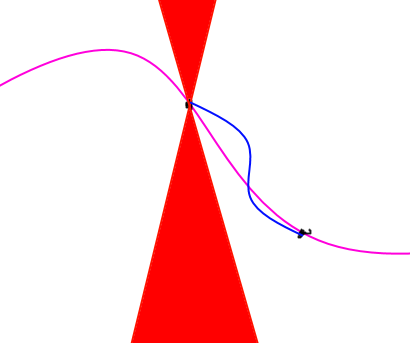
\includegraphics[width=0.4\textwidth]{graph_cone}
\end{figure}

If $x'$ is close to $x$, then there must be a geodesic $y$ connecting $(x, \omega(x))$ to $(x', \omega(x'))$ and such a geodesic must satisfy the negation of (\ref{estimate on vector field})
and therefore (\ref{derivative bounds}) must hold.
\end{proof}

\begin{lemma}\label{volume form is Lagrangian}
Let $N$ be a $C^1$ hypersurface in $M$, such that there exists a Killing foliation $\chi$ associated to a triple $(H, \partial_0, P)$ and a $C^1$ function $\omega$ whose graph is $N$, c.f. (\ref{N is a graph}).
Let $\vol_N$ be the volume form induced on $N$ by $g$, and let $\varphi(x) = (x, \omega(x))$ be the induced diffeomorphism $H \to N$.
Then:
\begin{enumerate}
\item The area Lagrangian $\Lagrange$ associated to $(H, X, P)$ satisfies
\begin{equation}\label{volume form pullback}
\varphi^* \vol_N = \Lagrange(d\omega).
\end{equation}
\item Let $\partial_1, \dots, \partial_{d - 1}$ be (the translates by $\partial_0$ of) a quasieuclidean frame on $H$. Then
$$\varphi^*(u_{,\mu} ~\vol) = \lambda^d (\delta_\mu^0 - \delta^i_\mu \omega_{,i}) ~\vol_h.$$
\end{enumerate}
\end{lemma}
\begin{proof}
Since $\partial_0$ is a Killing field,
\begin{equation}\label{preservation of scalar field}
0 = \delta^\lambda_0 g_{\mu \nu,\lambda} + \delta^\lambda_{0,\mu} g_{\nu\lambda} + \delta^\lambda_{0,\nu} g_{\mu \lambda} = g_{\mu\nu,0},
\end{equation}
so the scalar field $g_{\mu\nu}$ is preserved by $\varphi^*$.
Moreover, since $\partial_0$ is assumed normal to $H$, $g_{0i} = 0$.
If we write $\slashed g$ for the metric induced by $g$ on $N$, then
$$\varphi^* \vol_N = \varphi^* \sqrt{\det \slashed g} ~dx = \sqrt{\varphi^* \det \slashed g} ~dx.$$
From Lemma \ref{cross product formula} with $\psi = d\omega$, we obtain
\begin{align*}
\varphi^* \vol_N &= \lambda\sqrt{1 + |d\omega|_{h^{-1}}^2} \sqrt{\det h} ~dx = \Lagrange(d\omega)
\end{align*}
which proves (\ref{volume form pullback}).
Using (\ref{volume form pullback}, \ref{preservation of scalar field}) and the fact that $N$ is $C^1$, we fix a small open set $S$ and compute
\begin{align*}
\int_S u_{,\mu} ~\vol &= \int_{S \cap N} \normal_\mu ~\vol_N \\
&= \int_{\varphi^{-1}(S \cap N)} \sqrt{\frac{g_{00}}{1 + |\psi|_{h^{-1}}^2}} (\delta_\mu^0 - \delta_\mu^i \omega_{,i})\Lagrange(d\omega) \\
&= \int_{\varphi^{-1}(S \cap N)} \lambda^d (\delta_\mu^0 - \delta_\mu^i \omega_{,i}) \vol_h \qedhere.
\end{align*}
\end{proof}

\begin{notation}
Write $A(\rho)f = f(h, B_\rho, \Psi)$ for a $1$-form $f$ on $H$, where $B_\rho = B_h(P, \rho)$.
\end{notation}

\begin{lemma}\label{excess vs MVP}
In the situation of Lemma \ref{volume form is Lagrangian}, with $\Psi$ the trivialization of $T^* H$ induced by $\partial_1, \dots, \partial_{d - 1}$, $\Lambda_\Psi(U, r)$ is an element of the closed interval
$$\left[(1 - O(c))\int_{B_r} \Lagrange(dw) - \sqrt{1 + |A(\rho)d\omega|^2}\vol_h, (1 + O(c)) \int_{B_r} \Lagrange(dw) - \sqrt{1 + |A(\rho)d\omega|^2}\vol_h\right]$$
where the implied constant is absolute.
\end{lemma}
\begin{proof}
TODO: Prove it! Also we haven't actually defined $c$ yet so this is putting the cart before the horse, but that's easy to fix
\end{proof}

%%%%%%%%%%%%%%%%%%%%%%%%%%%%%%%%%%%%%%%%%%%%%

\subsection{Deforming the mean-value property}
Our next task is to show that the area Lagrangian (\ref{area Lagrangian}) satisfies an approximate mean-value property, which gives an improvement on \cite[Teorema 4.3]{Miranda66}.
TODO: Rewrite this to account for $A(\rho)$.

\begin{notation}
Let $(H, h, P)$ be a pointed Riemannian manifold of dimension $d - 1$.
We define a metric $\tilde h$ with vanishing curvature by considering normal coordinates $x_1, \dots, x_{d - 1}$ with respect to $h$ and setting $\tilde h_{ij} = \delta_{ij}$, thus
$$h_{ij} = \tilde h_{ij} + O(x^2)$$
where the implied constant depends continuously on $h$ and its derivatives at $P$.
We then define the $\tilde h$-Dirichlet energy
$$\DirL(\psi) = \frac{\tilde h^{ij} \psi_i \psi_j}{2}\vol_{\tilde h}.$$
Let $B_r$ denote a ball centered on $P$ in the euclidean space $(H, \tilde h)$, not in $M$.
Let $A(r)f$ denote the $\tilde h$-mean of $f$ over $B_r$.
Note that we can take means of $1$-forms as well as functions, since $\tilde h$ is flat.
\end{notation}

\begin{lemma}\label{Taylor lemma}
Let $(H, h, P)$ be a pointed Riemannian manifold of dimension $d - 1$, let $\lambda$ be a scalar field on $H$, let $\Lagrange$ satisfy (\ref{area Lagrangian}), and suppose that there exists $c \in (0, 1)$ such that for every $1$-form $\psi$,
\begin{align}
1 - c \leq |\lambda|, g_{00} \leq 1 + c, \label{estimate on Killing weight} \\
1 - c \leq \frac{|\psi|^2_{h^{-1}}}{|\psi|^2_{\tilde h^{-1}}} \leq 1 + c, \label{estimate on normal coordinates}\\
1 - c \leq \sqrt{\frac{\det h}{\det \tilde h}} \leq 1 + c, \label{estimate on normal volume form}
\end{align}
If $p,q$ are $1$-form on $H$ such that $|q|^2_{h^{-1}} \lesssim 1$, then $\Lagrange(p) - \Lagrange(q)$ lies in the closed interval
$$\left[\frac{1 - O(c)}{\Lagrange(q)}(\DirL(p) - \DirL(q)) - O(\DirL(p) - \DirL(q))^2, (1 + O(c))(\DirL(p) - \DirL(q))\right]$$
where all implied constants are absolute.
\end{lemma}
\begin{proof}
Let $\DirL_h(Y) = \sqrt{1 + h_{ij} Y^i Y^j}/2 ~\vol_h$ be the Dirichlet energy with respect to $h$.
Applying (\ref{estimate on normal coordinates}, \ref{estimate on normal volume form}),
\begin{equation}\label{estimate on normal coordinates 2}
1 - O(c) \leq \frac{\DirL(p) - \DirL(q)}{\DirL_h(p) - \DirL_h(q)} \leq 1 + O(c).
\end{equation}
By Taylor's theorem, there exists $\xi \geq 0$ between $|p|$ and $|q|$ such that
\begin{align*}
\lambda^{-1}(\Lagrange(p) - \Lagrange(q)) &= \sqrt{1 + |p|^2} - \sqrt{1 + |q|^2}\\
&= \frac{|p|^2 - |q|^2}{2 \sqrt{1 + |q|^2}} - \frac{(|p|^2 - |q|^2)^2}{8(1 + \xi^2)^{3/2}} \\
&= \frac{\DirL_h(p) - \DirL_h(q)}{\sqrt{1 + |q|^2}} - \frac{(\DirL_h(p) - \DirL_h(q))^2}{2(1 + \xi^2)^{3/2}}.
\end{align*}
Since $|q|^2 \geq 0$ and the second term is nonpositive, it follows from (\ref{estimate on Killing weight}, \ref{estimate on normal coordinates 2}) that
$$\Lagrange(p) - \Lagrange(q) \leq (1 + c)(\DirL_h(p) - \DirL_h(q)) \leq (1 + O(c))(\DirL(p) - \DirL(q)).$$
If $|q|^2_h$ is small enough,
$$2\Lagrange(q) \leq 8 \leq 8(1 + \xi^2)^{3/2},$$
whence
\begin{align*}
\frac{(1 + c)^{-1}(\DirL(p) - \DirL(q))}{\Lagrange(q)} - \frac{2(1 + c)^{-2}(\DirL(p) - \DirL(q))^2}{\Lagrange(q)} &\leq \Lagrange(p) - \Lagrange(q).
\end{align*}
Another application of (\ref{estimate on normal coordinates 2}) completes the proof.
\end{proof}

\begin{lemma}\label{Dirichlet}
For every $c \in (0, 1)$ there exists $\rho^* = \rho^*(c, g, P) > 0$ which depends continuously on $P$ and with the following property.

Let $H$ be a hypersurface which is normal to a Killing field, and for which $\chi,\Lagrange$ are given by Definition \ref{Killing setup}.
Let $\omega: H \to \RR$ be $C^1$, and suppose that $U \subseteq M$ is an open set such that
$$\partial U = \{\chi(x, \omega(x)): x \in H\}.$$
Then for every $\rho \in (0, \rho^*)$ and $\alpha, \kappa, \beta \in (0, 1)$ such that
\begin{align}
||d\omega||_{L^\infty(B_\rho)} &\leq \kappa, \label{Dirichlet small derivative}\\
\int_{B_\rho} \Lagrange(d\omega) - \Lagrange(A(\rho)d\omega) &\leq \beta, \label{Dirichlet close to mean} \\
\int_{B_\rho} \Lagrange(d\omega) &\leq \eta(U, \rho) + \beta \kappa, \label{Dirichlet close to minimal}
\end{align}
it follows that
\begin{equation}\label{Dirichlet gain}
\int_{B_{\alpha\rho}} \Lagrange(d\omega) - \Lagrange(A(\alpha\rho)d\omega) \leq (1 + O(c))\alpha^{d + 1}\beta + O(\beta \kappa^{1/2})
\end{equation}
where all implied constants are absolute.
\end{lemma}
The role of these parameters is as follows: we will take $\beta,\kappa \to 0$ in a proof by compactness and contradiction, and when we apply Proposition \ref{mollifier proposition}, we will take $\alpha \to 1/2$. One should think of $\beta$ as much smaller than $\kappa$, which in turn is much smaller than $c,\alpha,\rho^*$.
Indeed, $c$ will later be chosen absolutely, so $\rho^*$ only depends on $P,g$.
Once we have fixed $\rho^*$, we will iteratively halve the scale $\rho$ so that we can capitalize on (\ref{Dirichlet gain}).
\begin{proof}
Let $h,\lambda$ be as in Definition \ref{Killing setup}.
Then $\lambda(P) = 1$ and $\lambda$ depends only on $g,P$.
So we can use (\ref{Dirichlet small derivative}) and the fact that $\kappa < 1$ to select $\rho^*$ independently of $\omega$, so that such that
if $\rho < \rho^*$, then $\lambda$ is controlled by (\ref{estimate on Killing weight}),
$h$ is controlled by (\ref{estimate on normal coordinates}, \ref{estimate on normal volume form}), and
$$||d\omega||_{L^\infty(B_\rho)} \cdot |B_\rho| \lesssim 1.$$
Thus we will be able to apply Lemma \ref{Taylor lemma}.
Since $h$ is of the form $h(v, w) = g(X, X)^{-1} g(v, w)$ for a Killing field $X$, and the space of Killing fields defined near $P$ is finite-dimensional, $h$ and its derivatives are all controlled by $g,P$ and so $\rho^*$ is determined by $c,P,g$.

Let $u$ be the $\tilde h$-harmonic function on $B_\rho$ such that $u|\partial B_\rho = \omega|\partial B_\rho$.
By definition of $\eta(U, \rho)$ and (\ref{Dirichlet close to minimal}),
\begin{equation}\label{Dirichlet close to harmonic}
\int_{B_\rho} \Lagrange(d\omega) - \Lagrange(\nabla u) \leq \int_{B_\rho} \Lagrange(d\omega) - \eta(U, \rho) \leq \beta\kappa.
\end{equation}
We now proceed analogously to the proof of \cite[Lemma 4.2]{Miranda66}. By Lemma \ref{Taylor lemma},
\begin{align*}
\int_{B_{\alpha\rho}} \Lagrange(d\omega) - \Lagrange(A(\alpha\rho)d\omega) &\leq (1 + c)\int_{B_{\alpha\rho}} \DirL(d\omega) - \DirL(A(\alpha\rho)d\omega) \\
&= \frac{1 + c}{2} \int_{B_{\alpha\rho}} |d\omega|^2 - |A(\alpha\rho)d\omega|^2.
\end{align*}
Since $A(\alpha\rho)d\omega$ is the mean of $d\omega$, we have for every $\varepsilon > 0$
\begin{align*}
\int_{B_{\alpha\rho}} |d\omega|^2 - |A(\alpha\rho)d\omega|^2 &\leq \int_{B_{\alpha\rho}} (d\omega - A(\rho)d\omega)^2 ~dx \\
&\leq (1 + \varepsilon^{-1})\int_{B_\rho} |d\omega - \nabla u|^2 ~dx\\
&\qquad + (1 + \varepsilon) \int_{B_{\alpha\rho}} |\nabla u - A(\rho)d\omega|^2 ~dx\\
&=: O(\varepsilon^{-1})I + (1 + \varepsilon)J.
\end{align*}
To estimate $I$, we use the mean-value property, Lemma \ref{Taylor lemma}, and (\ref{Dirichlet close to harmonic}):
\begin{align*}
I &= \int_{B_\rho} |d\omega - \nabla u|^2 = \int_{B_\rho} |d\omega|^2 - |\nabla u|^2 \lesssim \int_{B_\rho} \Lagrange(d\omega) - \Lagrange(\nabla u) \leq \beta \kappa.
\end{align*}
To estimate $J$, we apply \cite[Lemma 4.1]{Miranda66}:
\begin{align*}
J &= \int_{B_\rho} |\nabla u|^2 - |A(\rho)d\omega|^2 = \int_{B_\rho} |\nabla u|^2 - |A(\rho)\nabla u|^2 \\
&\leq \alpha^{d + 1} \int_{B_\rho} |\nabla u|^2 - |A(\rho)\nabla u|^2 \leq \alpha^{d + 1} \int_{B_\rho} |d\omega|^2 - |A(\rho)d\omega|^2 \\
&\leq \alpha^{d + 1} \int_{B_\rho} |d\omega - A(\rho)d\omega|^2 ~dx \\
&\leq (1 + \varepsilon)\alpha^{d + 1} \int_{B_\rho} |d\omega - A(\rho)d\omega|^2  + O(\varepsilon^{-1})\int_{B_\rho} |d\omega - \nabla u|^2\\
&=: (1 + \varepsilon)\alpha^{d + 1}K + O(\varepsilon^{-1})I.
\end{align*}
We already estimated $I \lesssim \beta \kappa$, and now we estimate $K$: by Lemma \ref{Taylor lemma} and (\ref{Dirichlet small derivative}, \ref{Dirichlet close to mean}),
\begin{align*}
K &= \int_{B_\rho} |d\omega|^2 - |A(\rho)d\omega|^2\\
&\leq 2\int_{B_\rho} \DirL(d\omega) - \DirL(A(\rho)d\omega)\\
&\leq 2(1 + O(c))\int_{B_\rho} \Lagrange(d\omega) - \Lagrange(A(\rho)d\omega) + O(1) \int_{B_\rho} (\DirL(d\omega) - \DirL(A(\rho)d\omega))^2\\
&\leq 2(1 + O(c))\beta + O(1) ||d\omega||_{L^\infty(B_\rho)} \int_{B_\rho} \DirL(d\omega) - \DirL(A(\rho)d\omega) \\
&\leq 2\beta(1 + O(c + \kappa)).
\end{align*}
If we set $\varepsilon = \kappa^{1/2}$ then we conclude
\begin{align*}
\int_{B_{\alpha\rho}} \Lagrange(d\omega) - \Lagrange(A(\alpha\rho)d\omega)
&\leq (1 + O(c + \varepsilon)) \alpha^{d + 1}\beta + O(\beta \kappa \varepsilon^{-1})\\
&\leq (1 + O(c))\alpha^{d + 1} \beta + O(\beta \kappa^{1/2}). \qedhere
\end{align*}
\end{proof}

\subsection{\texorpdfstring{$C^1$}{C1} case}
With the above setup, we now are ready to show the $C^1$ case of de Giorgi's lemma \cite[Teorema 4.4]{Miranda66}.

\begin{lemma}\label{DGLC1}
Suppose that $M$ is a locally homogeneous Riemannian manifold, $U$ is a set of least perimeter, $\normal = \normal_U$, $\beta, \kappa, c > 0$, and $P \in \partial^* U$.
Let $(H, X)$ be the tangent hypersurface and Killing field induced by $(M, P)$ (c.f. Lemma \ref{hopfKilling}), and let $\Psi$ be the trivialization of $T^* H$ induced by a quasieuclidean frame on $(H, P)$ (c.f. Lemma \ref{extend to quasieuclid}).
If $\rho < \rho^*$ where $\rho^* = \rho^*(c, P, g)$ depends continuously on $P$, and
\begin{align}
||\normal^\sharp - X||_{L^\infty(B_\rho)} \leq \kappa^2, \label{DGLC1 normal points up} \\
|\partial U \cap B(P, \rho)| \leq \eta(U, B(P, \rho)) + \beta \kappa, \label{DGLC1 almost minimal} \\
\Lambda_\Psi(U, \rho) \leq \beta, \label{DGLC1 small excess}
\end{align}
then 
\begin{equation}
\Lambda_\Psi(U, \rho/2) \leq \frac{1 + O(c)}{2^{d + 1}} \beta + O(\beta \kappa^{1/2}) \label{DGLC1 conclusion}
\end{equation}
where all implied constants are absolute.
\end{lemma}
\begin{proof}
Using Lemma \ref{hopfKilling}, there exists a Killing foliation $\chi$ associated to $(H, X)$, an open submanifold $M' \subseteq M$, and a $C^1$ function
$$\omega: H \cap M' \to \RR$$
such that $N = \partial U \cap M'$ equals $\{(x, \omega(x)): x \in H \cap M'\}$, $\omega(x) = 0$, and 
$$||d\omega||_{L^\infty(B(P, \rho))} \lesssim ||(\normal, X) - (X, X)||_{L^\infty(B(P, \rho))}^{1/2}.$$
The space of Killing fields is finite-dimensional and so has a compact $L^\infty$-unit ball; therefore we can choose $\rho^*$ independently of $U$ so that $||X||_{L^\infty(B(P, \rho^*))} \leq 2$, in which case (\ref{DGLC1 normal points up}) gives
\begin{equation}\label{DGLC1 small derivative}
||d\omega||_{L^\infty(B(P, \rho))} \leq A\kappa
\end{equation}
for some absolute constant $A > 0$. If we assume that $\kappa < 1/A$, then it follows that 
$$||\omega||_{L^\infty(B(P, \rho))} < \rho ||d\omega||_{L^\infty(B(P, \rho))} \leq \rho.$$
Therefore $N \subseteq S_\rho$ and using the comparability of norms (TODO: Fill in the annoying details here) we may replace $B(P, \rho)$ with $S_\rho$.
From Lemma \ref{volume form is Lagrangian} and (\ref{DGLC1 almost minimal}),
$$\int_{B_\rho} \Lagrange(d\omega) \leq \eta(U, B(P, \rho)) + \beta \kappa$$
and Lemma \ref{excess vs MVP}, (\ref{DGLC1 small excess}) gives 
$$\int_{B_\rho} \Lagrange(d\omega) - \sqrt{1 + |A_\Psi(\rho)d\omega|^2} \leq (1 + O(c)) \beta$$
where the constant is absolute.
We may therefore apply Lemma \ref{Dirichlet} and (\ref{DGLC1 small derivative}) to obtain
$$\int_{B_{\rho/2}} \Lagrange(d\omega) - \sqrt{1 + |A_\Psi(\rho)d\omega|^2} \leq \frac{1 + O(c)}{2^{d + 1}} \beta + O(\beta \kappa^{1/2}) \beta$$
and another application of Lemmata \ref{volume form is Lagrangian}, \ref{excess vs MVP} now gives (\ref{DGLC1 conclusion}).
\end{proof}

\subsection{Removing the \texorpdfstring{$C^1$}{C1} assumption}\label{proof of DGL}
We are now ready to prove Proposition \ref{de Giorgi lemma}, and also settle the choice of $c > 0$.
By local homogeneity, if we can find $\sigma = \sigma(P)$, then $\sigma$ is locally constant and hence constant, so we may restrict to any particular $P \in M$.
Let $U$ be a set of locally finite perimeter, $u = 1_U$, and $\Psi$ a Killing frame.
Let $v_r = a^{-1}\int_{B_\rho} d_\Psi u ~\vol$, $a = |\int_{B_\rho} d_\Psi u ~\vol|$, so $v \in \RR^d$ has unit length and we can find an orthogonal matrix $O$\footnote{Note carefully that $O$ is \emph{not} a section of the $(1,1)$-tensor bundle: it is a constant matrix.} with $Ov = \evect^0$.
We then define $\Psi' = (\partial_\mu')$ where $\partial_\mu' = O^\nu_\mu \partial_\nu$, so that 
$$\int_{B_\rho} \partial_\mu'u~\vol = O^\nu_\mu \int_{B_\rho} \partial_\nu u ~\vol = aO^\nu_\mu v_\nu = a\delta_\mu^0.$$
Suppose that $R$ is small enough that $1/2 \leq g(\partial_\mu', \partial_\mu') \leq 2$ on $B_R$.

Let $\gamma^* > 0$ be the constant from Proposition \ref{mollifier quant} with $\delta = \rho$, and suppose that $\sigma \leq \gamma^*$ and $R$ is less than the injectivity radius of $M$.
Then for almost every $t \in (0, \rho)$, there exists a set $V \subseteq B_t$ with $C^1$ perimeter and satisfying (\ref{mollifier quant1}, \ref{mollifier quant2}, \ref{mollifier quant3}, \ref{mollifier quant4}) with $X = \partial_0'$.
It follows that $V$ satisfies (\ref{DGLC1 normal points up}, \ref{DGLC1 almost minimal}) with $B_\rho$ replaced by $B_t$ and $\beta \geq \rho^{d - 1} \gamma$, $\kappa = \varepsilon^{1/2}$.
From (\ref{mollifier quant2}, \ref{mollifier quant3}),
$$|\Lambda(U, t) - \Lambda(V, t)| \lesssim \varepsilon \rho^{d - 1} \gamma.$$
Therefore, (\ref{DGLC1 small excess}) also holds for $V, B_t$ with
$$\beta = \rho^{d - 1} \gamma(1 + O(\varepsilon)).$$
Let $\rho^* > 0$ be the constant from Lemma \ref{DGLC1} and suppose that $R < \rho^*$.
Then
$$\Lambda(V, \rho/2) \leq \frac{1 + O(c + c\varepsilon^{1/4})}{2^{d + 1}} \beta,$$
so putting everything together, we find an absolute constant $b > 0$ such that if $t < \rho$ is large enough depending on $\varepsilon$,
$$\Lambda(U, \rho/2) \leq \frac{1 + b(c + c\varepsilon^{1/4} + \varepsilon)}{2^{d + 1}} \Lambda(U, \rho/2).$$
We may now choose $c, \varepsilon$ so small depending on $b$ that 
$$\Lambda(U, \rho/2) \leq 2^{-d} \Lambda(U, \rho)$$
which was to be shown.